%Latex->ps->pdf
%\documentclass{beamer}
\documentclass[handout]{beamer}
\newcommand{\ds}{\displaystyle}
\newcommand{\N}{\ensuremath{\mathbb{N}}}
\newcommand{\Nnul}{\ensuremath{\mathbb{N}_0}}
\newcommand{\RR}{\ensuremath{\mathbb{R}}}
\newcommand{\perdef}{\overset{\mathrm{def}}{=}}
\usepackage{amsmath,amssymb}
%\usepackage[latin1]{inputenc}
\usepackage{fancybox}
\usepackage{epic,overpic}

\usepackage{etex}
\usepackage[dutch]{babel}
\usepackage{hyphenat}
\usepackage{amsmath}
\usepackage{amssymb}
\usepackage{amsfonts}
\usepackage{graphicx}

\usepackage{color}
%\usepackage[thmmarks,framed,amsmath]{ntheorem}
\usepackage{answers}

\usepackage{framed}

\usepackage{pst-all}
\usepackage{epic}
\usepackage{eepic}
\usepackage{array}
\usepackage{booktabs}
\usepackage{multirow}
\usepackage{color}



%\usepackage{color}
%\usepackage[thmmarks,framed,amsmath]{ntheorem}


%\title{Voorkennisles 2}

\author{Annouk Van Vlierden}
\date{2018-2019}
%\usetheme{Montpellier}
\usetheme{CambridgeUS}
\usecolortheme{seahorse}

\begin{document}
\begin{frame}{Absolute waarde}
Voor een re\"eel getal
$a\in \RR$ defini\"eren we de \emph{ absolute waarde} van $a$
als \\$$|a|\overset{def}{=}\displaystyle\ \left\{\begin{array}{rll  } a & \mbox{als}& a \geqslant 0, \\
-a & \mbox{als} & a<0.\\
\end{array}\right.$$
\begin{itemize}
	\item Voorbeelden: $|5|=5,\; |-\pi|=\pi$ en $|1-\sqrt{2}|=\sqrt{2}-1$
	\item Eigenschap: Als $x \in \RR$ en $r>0 $, dan geldt: $|x|<r\qquad \Leftrightarrow
\qquad -r<x<r$
\end{itemize}
\end{frame}
\begin{frame}{Eigenschappen ongelijkheden}
 Voor elke $x,y,z \in\RR $ geldt
\begin{enumerate}
\item $x< y \;\Leftrightarrow \;x+z< y+z$.
\item $(x<y $ en $ \displaystyle z>
0)\; \Leftrightarrow \; xz< yz$.
\item $(x< y $ en $ \displaystyle z<0)\; \Leftrightarrow \; xz>
yz$.
\end{enumerate}

\end{frame}

\begin{frame}{Een functie toepassen op beide leden van een
ongelijkheid}
Kwadrateren
\begin{center}

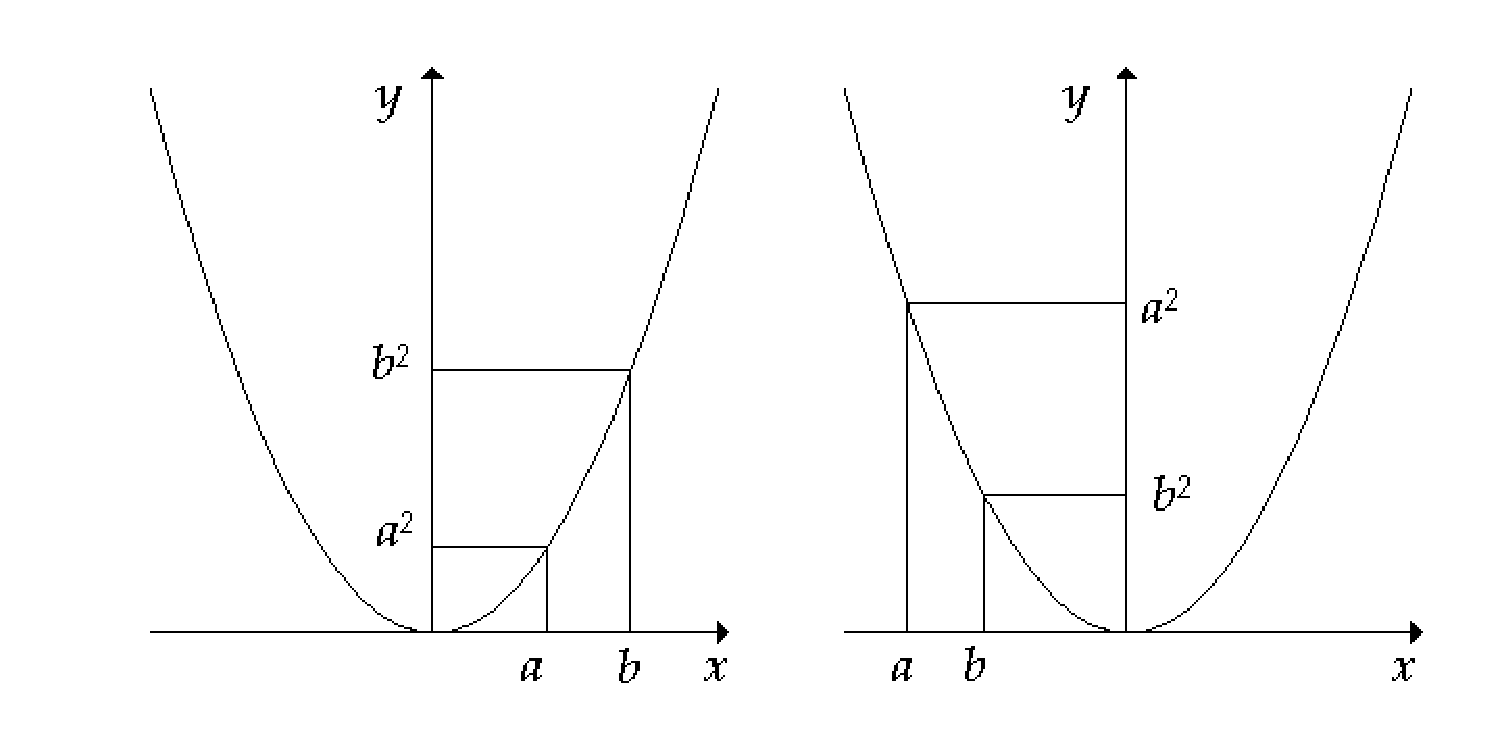
\includegraphics[width=9cm]{parabool2bis.ps}\end{center}

$$\mbox{als }a,b \geqslant 0, \mbox{ dan geldt } a<b\Leftrightarrow
a^2<b^2$$
$$\mbox{als }a,b \leqslant 0, \;\mbox{ dan
geldt } \;a<b\Leftrightarrow a^2>b^2$$

Als $a<0<b \;\mbox{ kan je niet weten of }\;a^2<b^2,\; \mbox{ofwel}
\;a^2>b^2$.
\end{frame}

\begin{frame}
{Ontbinden in factoren}
Een derdegraadsveelterm $f(x) = b x^3+ c x^2+ d x+ e$ ontbinden in
factoren van zo laag mogelijke graad: \begin{itemize} \item Stap 1:
Zoek een nulpunt $a$ van $f(x)$. Dan kunnen we $f(x)$ schrijven als
$f(x) = (x-a) Q(x)$ met $Q(x)$ een tweedegraadsveelterm.
\item Stap 2: Bereken $\ds Q(x) = \frac{f(x)}{x-a}$
\item Stap 3: Ontbind $Q(x)$ verder in factoren indien mogelijk
\end{itemize}
Eig:  Als $b x^3+ c x^2+ d x+ e$, met $b$,$c$, $d$, $e$ gehele
getallen, deelbaar is door $(x-a)$, met $a$ geheel, dan moet $a$ een
deler zijn van de constante term $e$. Indien $f(x)$ geen enkel
geheel nulpunt heeft dan moeten we een benaderingsmethode gebruiken
(zie Hoofdstuk 5)
\end{frame}
\end{document}

